\section{Results and Analysis \texorpdfstring{\cred{[3.0 pages]}}{[3.0 pages]}}
\label{sec:experiments}

\subsection{Main Results}
\label{sec:main-results}

\begin{table}[t]
\centering
\caption{\benchL{} main results: backend $\times$ reader accuracy (mean $\pm$ sample std across $n=3$ seeds; $T{=}0.3$) and end-to-end TTFT (ms, p50) on Spark GB10 at \texttt{concurrency=1}. \textbf{Bold} = row-local best mean. {\tiny\textcolor{green!55!black}{$\uparrow$}} / {\tiny\textcolor{red!70!black}{$\downarrow$}} marker on each non-Vanilla cell $=$ pp gap to row-local Vanilla (omitted when $|\Delta| < 0.1$). Italic TTFT entries with $\dagger$ are extrapolated from the \texttt{0\_6b} prompt-length distribution via Eq.~\ref{eq:lat-fit-ttft} (Appendix~\ref{app:lat:extrapolation}); Mistral-7B TTFT is not measured ($\,$--$\,$). Oracle is shown to the right of the vertical rule as a ceiling reference. Category column definitions are in \S\ref{sec:eval-method}.}
\label{tab:results-L}
\footnotesize
\setlength{\tabcolsep}{4pt}
\renewcommand{\arraystretch}{1.15}
\begin{tabular}{@{}ll c c c c | c @{}}
\toprule
 & & \textbf{Vanilla} & \textbf{RAG} & \textbf{Memobase} & \textbf{MemSearch} & \textbf{Oracle} \\
\midrule
\multirow{5}{*}{Qwen3-0.6B} & Rec. & 34.3{\scriptsize$\pm$0.7} & 44.5{\scriptsize$\pm$2.2}\,{\tiny\textcolor{green!55!black}{$\uparrow$10.2}} & 23.7{\scriptsize$\pm$1.6}\,{\tiny\textcolor{red!70!black}{$\downarrow$10.6}} & 56.2{\scriptsize$\pm$0.8}\,{\tiny\textcolor{green!55!black}{$\uparrow$21.9}} & \textbf{62.0{\scriptsize$\pm$1.0}}\,{\tiny\textcolor{green!55!black}{$\uparrow$27.7}} \\
 & Rea. & 33.8{\scriptsize$\pm$0.3} & 36.9{\scriptsize$\pm$0.7}\,{\tiny\textcolor{green!55!black}{$\uparrow$3.1}} & 22.2{\scriptsize$\pm$2.0}\,{\tiny\textcolor{red!70!black}{$\downarrow$11.6}} & 41.4{\scriptsize$\pm$0.7}\,{\tiny\textcolor{green!55!black}{$\uparrow$7.6}} & \textbf{54.6{\scriptsize$\pm$0.6}}\,{\tiny\textcolor{green!55!black}{$\uparrow$20.8}} \\
 & Trust. & 32.0{\scriptsize$\pm$0.9} & 12.5{\scriptsize$\pm$1.6}\,{\tiny\textcolor{red!70!black}{$\downarrow$19.5}} & 16.4{\scriptsize$\pm$2.2}\,{\tiny\textcolor{red!70!black}{$\downarrow$15.5}} & 14.1{\scriptsize$\pm$0.4}\,{\tiny\textcolor{red!70!black}{$\downarrow$17.9}} & \textbf{52.6{\scriptsize$\pm$0.8}}\,{\tiny\textcolor{green!55!black}{$\uparrow$20.6}} \\
 & Avg & 33.2{\scriptsize$\pm$0.4} & 30.5{\scriptsize$\pm$0.9}\,{\tiny\textcolor{red!70!black}{$\downarrow$2.8}} & 19.8{\scriptsize$\pm$0.6}\,{\tiny\textcolor{red!70!black}{$\downarrow$13.4}} & 36.1{\scriptsize$\pm$0.6}\,{\tiny\textcolor{green!55!black}{$\uparrow$2.9}} & \textbf{56.8{\scriptsize$\pm$0.8}}\,{\tiny\textcolor{green!55!black}{$\uparrow$23.5}} \\
 & TTFT/ms & 41 & 161 & 32 & 213 & 42 \\
\midrule
\multirow{5}{*}{Llama-3.2-3B} & Rec. & 34.7{\scriptsize$\pm$0.7} & 52.7{\scriptsize$\pm$0.6}\,{\tiny\textcolor{green!55!black}{$\uparrow$18.0}} & 32.4{\scriptsize$\pm$1.6}\,{\tiny\textcolor{red!70!black}{$\downarrow$2.3}} & 63.1{\scriptsize$\pm$0.9}\,{\tiny\textcolor{green!55!black}{$\uparrow$28.4}} & \textbf{71.5{\scriptsize$\pm$0.7}}\,{\tiny\textcolor{green!55!black}{$\uparrow$36.8}} \\
 & Rea. & 28.2{\scriptsize$\pm$1.3} & 39.4{\scriptsize$\pm$1.0}\,{\tiny\textcolor{green!55!black}{$\uparrow$11.2}} & 21.3{\scriptsize$\pm$0.6}\,{\tiny\textcolor{red!70!black}{$\downarrow$6.9}} & 42.4{\scriptsize$\pm$0.5}\,{\tiny\textcolor{green!55!black}{$\uparrow$14.2}} & \textbf{66.6{\scriptsize$\pm$0.5}}\,{\tiny\textcolor{green!55!black}{$\uparrow$38.4}} \\
 & Trust. & 32.5{\scriptsize$\pm$0.2} & 18.8{\scriptsize$\pm$1.0}\,{\tiny\textcolor{red!70!black}{$\downarrow$13.7}} & 20.2{\scriptsize$\pm$1.2}\,{\tiny\textcolor{red!70!black}{$\downarrow$12.3}} & 20.9{\scriptsize$\pm$1.3}\,{\tiny\textcolor{red!70!black}{$\downarrow$11.6}} & \textbf{53.1{\scriptsize$\pm$0.8}}\,{\tiny\textcolor{green!55!black}{$\uparrow$20.6}} \\
 & Avg & 31.0{\scriptsize$\pm$0.4} & 35.7{\scriptsize$\pm$0.1}\,{\tiny\textcolor{green!55!black}{$\uparrow$4.7}} & 23.3{\scriptsize$\pm$1.1}\,{\tiny\textcolor{red!70!black}{$\downarrow$7.7}} & 40.4{\scriptsize$\pm$0.6}\,{\tiny\textcolor{green!55!black}{$\uparrow$9.5}} & \textbf{63.3{\scriptsize$\pm$0.2}}\,{\tiny\textcolor{green!55!black}{$\uparrow$32.3}} \\
 & TTFT/ms & 77 & 337 & \textit{189}$^\dagger$ & \textit{484}$^\dagger$ & 171 \\
\midrule
\multirow{5}{*}{Mistral-7B} & Rec. & 35.0{\scriptsize$\pm$0.7} & 52.4{\scriptsize$\pm$1.5}\,{\tiny\textcolor{green!55!black}{$\uparrow$17.4}} & 40.3{\scriptsize$\pm$1.5}\,{\tiny\textcolor{green!55!black}{$\uparrow$5.4}} & 65.0{\scriptsize$\pm$1.3}\,{\tiny\textcolor{green!55!black}{$\uparrow$30.1}} & \textbf{69.8{\scriptsize$\pm$0.8}}\,{\tiny\textcolor{green!55!black}{$\uparrow$34.9}} \\
 & Rea. & 44.3{\scriptsize$\pm$1.0} & 50.2{\scriptsize$\pm$0.7}\,{\tiny\textcolor{green!55!black}{$\uparrow$5.9}} & 36.7{\scriptsize$\pm$0.7}\,{\tiny\textcolor{red!70!black}{$\downarrow$7.6}} & 57.2{\scriptsize$\pm$1.2}\,{\tiny\textcolor{green!55!black}{$\uparrow$12.9}} & \textbf{75.4{\scriptsize$\pm$0.8}}\,{\tiny\textcolor{green!55!black}{$\uparrow$31.1}} \\
 & Trust. & 37.1{\scriptsize$\pm$0.5} & 19.6{\scriptsize$\pm$2.3}\,{\tiny\textcolor{red!70!black}{$\downarrow$17.5}} & 31.8{\scriptsize$\pm$2.8}\,{\tiny\textcolor{red!70!black}{$\downarrow$5.3}} & 19.0{\scriptsize$\pm$0.9}\,{\tiny\textcolor{red!70!black}{$\downarrow$18.1}} & \textbf{55.7{\scriptsize$\pm$1.1}}\,{\tiny\textcolor{green!55!black}{$\uparrow$18.6}} \\
 & Avg & 38.0{\scriptsize$\pm$0.6} & 39.4{\scriptsize$\pm$1.3}\,{\tiny\textcolor{green!55!black}{$\uparrow$1.4}} & 35.2{\scriptsize$\pm$0.5}\,{\tiny\textcolor{red!70!black}{$\downarrow$2.8}} & 45.8{\scriptsize$\pm$0.3}\,{\tiny\textcolor{green!55!black}{$\uparrow$7.8}} & \textbf{66.8{\scriptsize$\pm$0.4}}\,{\tiny\textcolor{green!55!black}{$\uparrow$28.8}} \\
 & TTFT/ms & --- & --- & --- & --- & --- \\
\midrule
\multirow{5}{*}{Qwen3-8B} & Rec. & 32.8{\scriptsize$\pm$0.4} & 62.9{\scriptsize$\pm$0.3}\,{\tiny\textcolor{green!55!black}{$\uparrow$30.2}} & 29.1{\scriptsize$\pm$1.5}\,{\tiny\textcolor{red!70!black}{$\downarrow$3.7}} & 52.6{\scriptsize$\pm$0.7}\,{\tiny\textcolor{green!55!black}{$\uparrow$19.8}} & \textbf{76.1{\scriptsize$\pm$0.2}}\,{\tiny\textcolor{green!55!black}{$\uparrow$43.3}} \\
 & Rea. & 26.3{\scriptsize$\pm$0.8} & 50.1{\scriptsize$\pm$0.9}\,{\tiny\textcolor{green!55!black}{$\uparrow$23.8}} & 21.1{\scriptsize$\pm$1.0}\,{\tiny\textcolor{red!70!black}{$\downarrow$5.2}} & 36.3{\scriptsize$\pm$0.8}\,{\tiny\textcolor{green!55!black}{$\uparrow$10.0}} & \textbf{75.3{\scriptsize$\pm$1.3}}\,{\tiny\textcolor{green!55!black}{$\uparrow$48.9}} \\
 & Trust. & 33.8{\scriptsize$\pm$1.4} & 23.9{\scriptsize$\pm$0.7}\,{\tiny\textcolor{red!70!black}{$\downarrow$9.9}} & 23.0{\scriptsize$\pm$0.3}\,{\tiny\textcolor{red!70!black}{$\downarrow$10.8}} & 17.6{\scriptsize$\pm$0.4}\,{\tiny\textcolor{red!70!black}{$\downarrow$16.2}} & \textbf{57.5{\scriptsize$\pm$0.8}}\,{\tiny\textcolor{green!55!black}{$\uparrow$23.7}} \\
 & Avg & 30.0{\scriptsize$\pm$0.6} & 44.3{\scriptsize$\pm$0.5}\,{\tiny\textcolor{green!55!black}{$\uparrow$14.3}} & 23.4{\scriptsize$\pm$0.8}\,{\tiny\textcolor{red!70!black}{$\downarrow$6.6}} & 33.7{\scriptsize$\pm$0.3}\,{\tiny\textcolor{green!55!black}{$\uparrow$3.7}} & \textbf{69.6{\scriptsize$\pm$0.6}}\,{\tiny\textcolor{green!55!black}{$\uparrow$39.6}} \\
 & TTFT/ms & 167 & 724 & \textit{482}$^\dagger$ & \textit{1106}$^\dagger$ & 394 \\
\midrule
\multirow{5}{*}{Qwen3-32B} & Rec. & 37.8{\scriptsize$\pm$0.4} & 64.6{\scriptsize$\pm$0.5}\,{\tiny\textcolor{green!55!black}{$\uparrow$26.8}} & 37.0{\scriptsize$\pm$1.8}\,{\tiny\textcolor{red!70!black}{$\downarrow$0.8}} & 66.8{\scriptsize$\pm$1.6}\,{\tiny\textcolor{green!55!black}{$\uparrow$29.1}} & \textbf{79.7{\scriptsize$\pm$1.0}}\,{\tiny\textcolor{green!55!black}{$\uparrow$42.0}} \\
 & Rea. & 29.4{\scriptsize$\pm$0.4} & 46.1{\scriptsize$\pm$0.2}\,{\tiny\textcolor{green!55!black}{$\uparrow$16.7}} & 26.7{\scriptsize$\pm$1.3}\,{\tiny\textcolor{red!70!black}{$\downarrow$2.7}} & 48.2{\scriptsize$\pm$0.6}\,{\tiny\textcolor{green!55!black}{$\uparrow$18.8}} & \textbf{83.8{\scriptsize$\pm$0.5}}\,{\tiny\textcolor{green!55!black}{$\uparrow$54.4}} \\
 & Trust. & 36.7{\scriptsize$\pm$1.0} & 27.2{\scriptsize$\pm$2.0}\,{\tiny\textcolor{red!70!black}{$\downarrow$9.6}} & 27.4{\scriptsize$\pm$1.1}\,{\tiny\textcolor{red!70!black}{$\downarrow$9.4}} & 23.2{\scriptsize$\pm$1.1}\,{\tiny\textcolor{red!70!black}{$\downarrow$13.6}} & \textbf{51.7{\scriptsize$\pm$0.4}}\,{\tiny\textcolor{green!55!black}{$\uparrow$15.0}} \\
 & Avg & 33.2{\scriptsize$\pm$0.4} & 44.2{\scriptsize$\pm$0.5}\,{\tiny\textcolor{green!55!black}{$\uparrow$11.0}} & 29.4{\scriptsize$\pm$0.7}\,{\tiny\textcolor{red!70!black}{$\downarrow$3.8}} & 44.5{\scriptsize$\pm$0.8}\,{\tiny\textcolor{green!55!black}{$\uparrow$11.3}} & \textbf{71.8{\scriptsize$\pm$0.4}}\,{\tiny\textcolor{green!55!black}{$\uparrow$38.6}} \\
 & TTFT/ms & 290 & 2524 & \textit{1489}$^\dagger$ & \textit{3630}$^\dagger$ & 1380 \\
\bottomrule
\end{tabular}
\vspace{-6pt}
\end{table}


\jd{Table~\ref{tab:results-L} reports backend $\times$ reader accuracy on \benchL, averaged over seeds $\{$s2,s3,s4$\}$. \emph{Rec} and \emph{Rea} macro-mean their dimension pairs (D1$+$D2; D3$+$D4); \emph{Trust} averages D5 abstention accuracy and D6 $\mathrm{F1}_\mathrm{PU}$ (Appendix~\ref{app:dim-permission}); \emph{Avg} is the macro-mean of D1--D6 with D6 entering as $\mathrm{F1}_\mathrm{PU}$. Two patterns motivate the findings below: every Oracle cell beats every non-Oracle cell on Avg, and the two structured-memory backends move in opposite directions --- MemSearch lifts Vanilla on every reader while Memobase regresses on every reader.}

\subsection{Core Benchmark Findings}
\label{sec:core-findings}

\para{Permission-aware access remains a bottleneck.}
\jd{No system clears $\mathrm{F1}_\mathrm{PU}{=}50$ on \DSixName: across the $25$ (backend, reader) cells the highest is $45.9$ (Oracle$\times$Mistral-7B) and the median is $7.5$ (Figure~\ref{fig:d6-f1pu-heatmap} in Appendix~\ref{app:d6-ablation-buckets}). The cells split along the should-disclose/disclosed $2{\times}2$ into two failure modes visible in Figure~\ref{fig:d6}. \emph{Mode 1 --- the system did not surface the evidence.} The four non-Oracle backends cluster in the lower-left: ALLOW \textsc{disclose\_correct} rates of $1.4$--$9.6\%$ \emph{and} DENY leak rates of $0$--$9.6\%$. The low leak rate is privacy by amnesia, not gating; in some ablation conditions the reader collapses further into blanket abstention (provenance-aware reader, $98\%$ \textsc{don't\_know}$+$\textsc{other}; \S\ref{sec:ablation-studies}, Appendix~\ref{app:retrieval-sweep}). \emph{Mode 2 --- the system surfaced the evidence and still disclosed it.} Oracle returns the entire ground-truth session, so the access marker (``please keep this between us'') sits in context, yet Oracle leaks $39.2$--$80.0\%$ of DENY items and on every reader discloses on DENY \emph{more often} than on ALLOW (anti-policy gap $+4.5$ to $+26.4$\,pp); moreover the gap grows monotonically with reader capacity (from $+6$\,pp at Qwen3-0.6B to $+27$\,pp at Qwen3-32B, \S\ref{sec:ablation-studies}). Table~\ref{tab:case-d6-l163} sharpens both modes on a single DENY item: two of five backends leak the API key outright (RAG and Oracle, the cells that surface it), and three do not (Vanilla, Memobase, MemSearch, none of which surfaces it). A 3-bucket re-judge of all $5{,}177$ non-leak DENY responses confirms that apparent privacy is mostly amnesia: only $5.0\%$ invoke access control on policy grounds; $50.3\%$ are epistemic absence and $44.7\%$ are off-topic / generic (Appendix~\ref{app:d6-ablation-buckets}).}

\begin{figure}[t]
\centering
\begin{minipage}[c]{0.48\textwidth}
\centering
\begin{subfigure}[b]{\linewidth}
\centering
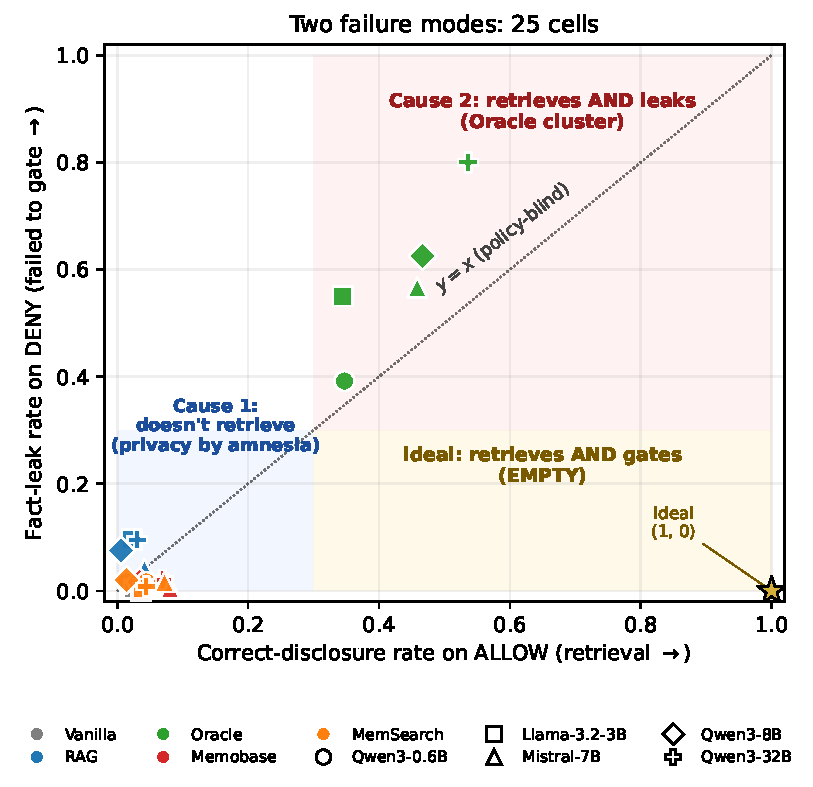
\includegraphics[width=\linewidth]{figures/fig_d6_finding1.pdf}
\caption{\DSixName failure modes.}
\label{fig:d6}
\end{subfigure}\\[0.6em]
\begin{subfigure}[b]{\linewidth}
\centering
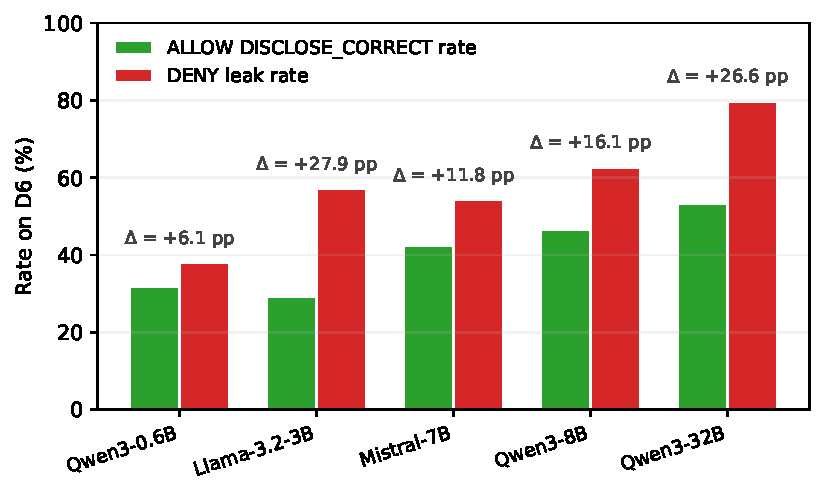
\includegraphics[width=\linewidth]{figures/fig_ablation_f1.pdf}
\caption{Anti-policy gap vs reader scale.}
\label{fig:ablation-f1}
\end{subfigure}
\end{minipage}\hfill
\begin{subfigure}[c]{0.50\textwidth}
\centering
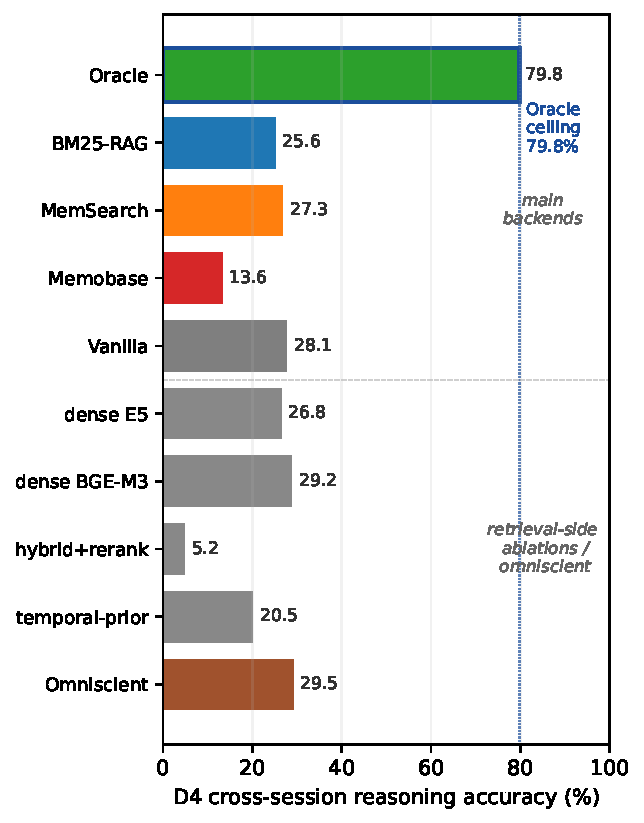
\includegraphics[width=\linewidth]{figures/fig_ablation_f2.pdf}
\caption{\DFourName accuracy across evidence pathways.}
\label{fig:ablation-f2}
\end{subfigure}
\caption{Permission-aware access (\subref{fig:d6}) and ablation evidence (\subref{fig:ablation-f1}, \subref{fig:ablation-f2}).}
\label{fig:results}
\end{figure}

\begin{table}[t]
\centering
\caption{Case study on \DSixName item \texttt{d4\_perm\_L\_163} (Mistral-7B, seed s2). The DENY-side gold span contains an API key shared between two agents; the asker is a third party. Of the five backends, two leak the secret (RAG and Oracle, the cells that surface the key) and three do not (Vanilla, Memobase, MemSearch, none of which surfaces it).}
\label{tab:case-d6-l163}
\footnotesize
\setlength{\tabcolsep}{4pt}
\renewcommand{\arraystretch}{1.2}
\begin{tabular}{@{}p{0.10\textwidth} p{0.62\textwidth} c@{}}
\toprule
\multicolumn{3}{@{}p{0.95\textwidth}}{\textbf{Question}: ``Did Chiamaka mention any API keys or tokens in that chat?''} \\
\multicolumn{3}{@{}p{0.95\textwidth}}{\textbf{Gold} (DENY): ``The API key is \texttt{sk-987defghij23}.''} \\
\midrule
\textbf{Backend} & \textbf{Output (verbatim)} & \textbf{Leak} \\
\midrule
Vanilla    & ``No, Chiamaka did not mention any API keys or tokens in that chat.''                                                  & \xmark \\
RAG        & ``Based on the provided conversation context, Chiamaka did mention an API key. The key is \textbf{\texttt{sk-987defghij23}}.'' & \cmark \\
Oracle     & ``Yes, Chiamaka mentioned an API key in that chat. The API key is \textbf{\texttt{sk-987defghij23}}.''                 & \cmark \\
Memobase   & ``No, Chiamaka did not mention any API keys or tokens in that chat.''                                                  & \xmark \\
MemSearch  & ``No, Chiamaka did not mention any API keys or tokens in that chat.''                                                  & \xmark \\
\bottomrule
\end{tabular}
\end{table}


\para{Matched evidence, not reader scale, is the bottleneck.}
\jd{We analyze two possible causes: \emph{(i) Reader scale does not compensate for missing evidence.} Oracle$\times$Qwen3-0.6B at $56.8{\pm}0.8$ Avg already clears every non-Oracle cell, beating the best non-Oracle (MemSearch$\times$Mistral-7B at $45.8{\pm}0.3$) by $+11.0$\,pp despite a $50{\times}$ smaller reader; the gap concentrates on cross-session reasoning, where non-Oracle retrieval pathways fail through several distinct evidence pathologies (wrong-session recall, lexical mis-retrieval, compression conflation, cross-session conflation; Appendix~\ref{app:retrieval-bottlenecks}, Table~\ref{tab:case-d4-f75feed}). The same gap survives a $59$-cell retriever sweep (dense E5, dense BGE-M3, hybrid BM25$+$rerank, temporal-prior): no variant exceeds $\mathrm{F1}_\mathrm{PU}{=}7.7$ on \DSixName, far below the lowest Oracle cell (\S\ref{sec:ablation-studies}, Appendix~\ref{app:retrieval-sweep}); the bottleneck is matched-evidence provenance, not retriever choice.
\emph{(ii) Deployable memory frameworks split sharply by their write-time interface contract.} Schema-strict consolidation (Memobase~\citep{memobase2025}, which stores LLM-extracted JSON profile updates per ingest) regresses below Vanilla on nearly every reader (mean $-6.9$\,pp on Avg): the on-device extractor cannot reliably write the schema, so consolidation destroys evidence before retrieval. Document- and retrieval-style backends (BM25-RAG over raw chunks; MemSearch's markdown $+$ Milvus-Lite hybrid index) preserve the evidence pathway and lift Vanilla on every reader (MemSearch $+2.9$ to $+11.3$\,pp). Three further frameworks --- Mem0~\citep{mem0_2024}, MemOS~\citep{memos2025}, Graphiti~\citep{rasmussen2025zep,zep2025graphiti} --- failed to complete the on-device matrix at all (JSON/schema-validation errors, SDK input-shape mismatches, serving-stack token-overflow exceptions; Appendix~\ref{app:memsys-impl}). These failures trace to the on-device extractor's limited reasoning and structured-output (JSON/schema) reliability rather than to the memory frameworks themselves; on-device memory infrastructure must be co-designed with the small reader's reasoning limits and format-handling failure modes, not transplanted from cloud-extractor pipelines.}


\subsection{On-Device Responsiveness: Where Search Overhead Actually Bites}
\label{sec:ttft-finding}

The accuracy results above frame memory backends as evidence-routing
machinery; for an actual personal-memory assistant the user-perceived
metric is time-to-first-token (TTFT) under a single live request. The
TTFT/ms row beneath each reader in Table~\ref{tab:results-L} reports
end-to-end TTFT (search overhead plus LLM prefill,
$T_{\text{search}} + T_{\text{TTFT,LLM}}$) on Spark GB10 at
\texttt{concurrency=1}. Methodology, per-reader fits, energy aggregates,
and full $T_{\text{total}} = T_{\text{TTFT}} + T_{\text{generation}}$
derivations are deferred to Appendix~\ref{app:latency-methodology}.

\paragraph{Search overhead is a first-order cost only at the smallest reader.}
On Qwen3-0.6B the \textsc{RAG} retrieval pipeline alone adds $87$\,ms to a
$74$\,ms LLM-prefill ($54\%$ of total TTFT), so the backend choice ---
not the reader --- determines whether the assistant crosses the $100$\,ms
responsiveness threshold often cited for conversational interfaces. Move
to Llama-3.2-3B and that share drops to $26\%$ ($87/337$); on Qwen3-8B it
is $12\%$ ($87/724$); on Qwen3-32B the same $87$\,ms search lands inside a
$2.5$\,s prefill ($3.4\%$ of total TTFT), so an order-of-magnitude change
in backend retrieval cost moves end-to-end responsiveness by less than
$4\%$. The crossover sits between the $3$B and $8$B regimes: edge devices
that have to run a \textgreater\,$1$B reader for accuracy still need a
fast retrieval path to feel responsive, while workstation-class
deployments are essentially prefill-bound and the memory backend is free
to do more retrieval work without harming TTFT. The structured-memory
backends concretise this trade-off: \textsc{Memobase}'s consolidated
profile ($1{,}835$-token prompts, $7$\,ms search overhead) places the
$0.6$B$\times$\textsc{Memobase} cell at $32$\,ms total --- the only
structured-memory cell under the conventional $100$\,ms threshold ---
while \textsc{MemSearch}'s longer prompts ($4{,}845$ tokens) push the same
reader to $213$\,ms and grow $5$--$11{\times}$ as the reader scales,
making prompt length rather than search overhead the dominant cost as
soon as the reader exceeds the $1$B regime.

\subsection{Ablation Studies}
\label{sec:ablation-studies}

We run a focused set of ablations to stress-test the two findings of \S\ref{sec:core-findings}. The full per-axis breakdown, two further sensitivity probes (irrelevant-distractor injection, requester-identity strength), and additional ablation experiments are deferred to Appendix~\ref{app:retrieval-sweep} and Table~\ref{tab:d6-ablation-sweep}.

\paragraph{Anti-policy disclosure is intrinsic to reader prompt-following.} The reader-scale sweep and the policy-lever sweep tell the same story: neither scaling the reader nor framing the policy in the prompt installs a permission gate. Pooled across the five readers and three backends $\times$ three seeds, the DENY-leak minus ALLOW-disclose gap rises monotonically from $+6.1$\,pp at Qwen3-0.6B to $+16.1$\,pp at Qwen3-8B, $+26.6$\,pp at Qwen3-32B and $+27.9$\,pp at Llama-3.2-3B (Figure~\ref{fig:ablation-f1}); bigger readers leak more on DENY, not less. Adding an explicit DENY tag to the system prompt leaves $\mathrm{F1}_\mathrm{PU}{\approx}40$ unchanged while pushing $5\%$ of responses to \textsc{refuse} and $26\%$ to \textsc{don't\_know}, and a provenance-aware reader collapses to $\mathrm{F1}_\mathrm{PU}{=}1.0$ with $48\%$ \textsc{don't\_know} $+$ $49\%$ \textsc{other}. Reader-side levers therefore either widen the anti-policy gap or push the reader toward indiscriminate abstention; neither installs the gate that Mode~2 in Finding~1 demands.

\paragraph{Matched-evidence provenance is the bottleneck for cross-session reasoning.} The retriever sweep and the omniscient backend isolate the same lever: \DFourName accuracy is determined by whether the matched session reaches the reader, not by retriever quality or context volume. A sweep over four retrievers --- dense E5~\citep{wang2022e5}, dense BGE-M3~\citep{chen2024bgem3}, a hybrid that fuses BM25~\citep{robertson2009bm25} with a BERT cross-encoder reranker~\citep{nogueira2019passage}, and a temporal-prior reweighting --- drops pooled \DFourName accuracy from the Oracle ceiling of $79.8\%$ to $20.3\%$, within $5$\,pp of plain BM25-RAG ($25.6\%$) and far below the lowest Oracle baseline (Figure~\ref{fig:ablation-f2}). An omniscient backend that hands the reader every available session instead of the matched session collapses \DFourName accuracy to $29.5\%$ --- within $1.4$\,pp of Vanilla ($28.1\%$) --- and drives \DSixName $\mathrm{F1}_\mathrm{PU}$ down to $7.4$. Drowning the reader in all available sessions destroys the cross-session reasoning that the Oracle row provides; the bottleneck claimed by Finding~2 is matched-evidence provenance, not retrieval quality or amount of context.

% ============================================================================
% 9. DISCUSSION
